\documentclass[12pt]{article}
\usepackage[utf8]{inputenc}
\usepackage[margin=1in]{geometry}
\usepackage[spanish]{babel}\decimalpoint
\usepackage{setspace}\onehalfspacing
\usepackage{parskip} % Espacio entre parrafos.
\usepackage{graphicx} % Para usar comando \includegraphics[]{}
\usepackage{tikz} % Visualizaciones.
\usepackage{amsmath, amssymb} % Extensión de símbolos y obj. matemáticos.
\usepackage{multirow} % Para unir multiples filas en una tabla.
\usepackage{hyperref} % Siempre debe ser el ultimo paquete.


\setcounter{tocdepth}{2} % Que no incluya subsubsections en la tabla de contenidos (toc).

%================================

\title{Clase 4. Ecuaciones de Planos y Sistemas Cuadrados de Ecuaciones.}
\author{MIT 18.02: Multivariable Calculus.}
\date{}


\begin{document}

\maketitle

\begin{abstract}
\noindent A partir de lo que hemos aprendido sobre vectores y matrices, profundizaremos sobre ecuaciones de planos y sistemas cuadrados de estos últimos. Estudiaremos la cantidad de soluciones que pueden tener tanto desde un enfoque geométrico como matricial, por medio del determinante de la matriz de coeficientes.
\end{abstract}


\section{Ecuaciones de Planos.}

Un \textbf{plano} en el espacio está definido por la siguiente ecuación lineal:
\[
  Ax + By + Cz = D
\]
donde $A$, $B$, $C$ y $D$ son constantes (o escalares).

Para conocer la ecuación de un plano, necesitamos \textbf{dos elementos}:

\begin{enumerate}
\item Un punto $P_{0} = (x_{0}, \ y_{0}, \ z_{0})$ por el cual pasa el plano\footnote{Es decir, es un punto que está en el plano.}.
\item Un vector $\mathbf{n}$ ortogonal al plano o \textbf{vector normal}.
\end{enumerate}

A nivel geométrico, la \textbf{dirección} del vector normal \textbf{indica el nivel de inclinación del plano}. En ese sentido, coincide con ser $\mathbf{n} = \langle A, \ B, \ C \rangle$.

Teniendo a $\mathbf{n}$ y a $P_{0}$, consideremos un segundo punto $P = (x, \ y, \ z)$ ubicado en cualquier lugar del plano y construyamos el vector:
\[
  \overrightarrow{P_{0}P} = \langle x - x_{0}, \ y - y_{0}, \ z - z_{0} \rangle
\]

\begin{figure}[hbt!]
\centering

\begin{tikzpicture}
% Celdas de ayuda
%\draw[help lines] (-5, -5) grid (5, 5);

% Origen.
\node at (-0.2, 0.1, 0) {$0$};

% Ejes x, y, z.
\draw [-latex, line width=0.3mm] (0, 0, 0) -- (3.5, 0, 0) node [below] {$y$}; % Original: eje X
\draw [-latex, line width=0.3mm] (0, 0, 0) -- (0, 3.5, 0) node [right] {$z$}; % Original: eje y
\draw [-latex, line width=0.3mm] (0, 0, 0) -- (0, 0, 3.5) node [below] {$x$}; % Original: eje z

% Plano.
\draw [blue, line width= 0.5mm, fill=cyan, opacity=0.8] (-2, 1) -- (1, 1.8) -- (3, -0.5) -- (0.1, -1.3) -- cycle;

% Vector Normal.
\draw [-latex, line width=0.4mm] (0.5, 1) -- (0.9, 2.2) node[above] {$\mathbf{n}$};

% Vector P_{0}P
\draw [red, -latex, line width=0.4mm] (0.23, -0.53) -- (-0.7, 0.5);
\node[text=red] at (0.25, 0.2) {$\overrightarrow{P_{0}P}$};

% Puntos.
\draw [fill=black] (0.3, -0.6) circle (1.1mm) node [right] {$P_{0}$};
\draw [fill=black] (-0.8, 0.6) circle (1.1mm) node [above] {$P$};

\end{tikzpicture}

\end{figure}

Como $\overrightarrow{P_{0}P}$ se ubica en el plano, entonces debe cumplirse que:
\[
  \mathbf{n} \cdot \overrightarrow{P_{0}P} = 0
\]
la cual recibe el nombre de \textbf{Ecuación Vectorial del Plano}. Al resolver el producto punto de su lado izquierdo obtenemos la \textbf{Ecuación Cartesiana del Plano}.
\begin{align*}
  \langle A, \ B, \ C \rangle \cdot \langle x - x_{0}, \ y - y_{0}, \ z - z_{0} \rangle &= 0 \\
  A(x - x_{0}) + B(y - y_{0}) + C(z - z_{0}) &= 0
\end{align*}
Para conocer la ecuación general del plano que vimos al inicio de esta sección, solo tenemos que continuar resolviendo el lado izquierdo de la ecuación cartesiana de la siguiente manera:
\begin{align*}
  Ax - Ax_{0} + By - By_{0} + Cz - Cz_{0} &= 0 \\
  Ax + By + Cz &= Ax_{0} + By_{0} + Cz_{0}
\end{align*}
La suma $Ax_{0} + By_{0} + Cz_{0}$ equivale al escalar $D$, porque $P_{0}$ y $\mathbf{n}$ están fijos en el espacio. Por lo tanto, podemos reescribir la ecuación cartesiana del plano como:
\[
  Ax + By + Cz = D
\]
\textbf{Ejemplo 1.} Encuentre la ecuación de un plano que pasa por el punto $P_{0}(2, \ 1, \ -1)$ y que tiene un vector normal $\mathbf{n} = \langle 1, \ 5, \ 10 \rangle$.

\textbf{Solución.} Usemos la fórmula de la ecuación cartesiana del plano para resolver este ejemplo, debido a que conocemos los componentes de $\mathbf{n}$ y las coordenadas de $P_{0}$, el cual se encuentra en esta figura.
\begin{align*}
  1 \cdot (x - 2) + 5 \cdot (y - 1) + 10 \cdot (z - (-1)) &= 0 \\
  x + 5y + 10z + 3 &= 0 \\
  x + 5y + 10z &= -3
\end{align*}

\textbf{Ejemplo 2.} Evalúe si el vector $\mathbf{v} = \langle 1, \ 2, \ -1 \rangle$ y el plano $x + y + 3z = 5$ son perpendiculares, paralelos o no poseen ninguna de las dos características entre sí.

\textbf{Solución.} Para resolver este ejemplo, podemos ayudarnos del vector normal del plano $x + y + 3z = 5$ el cual podemos garantizar que es $\mathbf{n} = \langle 1, \ 1, \ 3 \rangle$. Esto se debe a que si:

\begin{itemize}
\item $\mathbf{n} \perp \mathbf{v} \Longrightarrow \mathbf{v}$ es paralelo al plano.
\item $\mathbf{n} \parallel \mathbf{v} \Longrightarrow \mathbf{v}$ es ortogonal al plano.
\end{itemize}

Estas conjeturas podemos evaluarlas por medio del producto punto entre $\mathbf{n}$ y $\mathbf{v}$. Si
\[
 \mathbf{n} \cdot \mathbf{v} = 0,
\]
entonces son perpendiculares. En cambio, si
\[
  \mathbf{n} \cdot \mathbf{v} = \pm \left(||\mathbf{n}|| \cdot ||\mathbf{v}||\right)
\]
significa que son paralelos, lo cual se explica por el hecho de que el ángulo que se forma entre ellos es de $0$ (i.e, $0^{\circ}$) o $\pi$ (i.e, $180^{\circ}$). Esto implica que el $\cos(0) = 1$ o $\cos(\pi) = -1$, de ahí el cambio de signo que vemos arriba.

Calculemos primero el producto punto entre $\mathbf{v}$ y $\mathbf{n}$.
\[
  \mathbf{n} \cdot \mathbf{v} = \langle 1, \ 1, \ 3 \rangle \cdot \langle 1, \ 2, \ -1 \rangle = 1 + 2 - 3 = 0
\]
Por lo tanto, $\mathbf{n} \perp \mathbf{v}$, lo que significa que $\mathbf{v}$ es paralelo al plano $x + y + 3z = 5$

\subsection{Relevancia del Vector Normal.}

El elemento que nos entrega más información sobre un plano, es su vector normal. Anteriormente vimos que su dirección nos indica cómo está inclinado esta figura. En ese sentido, \textbf{si un vector es perpendicular en dos o más planos}, entonces estos últimos son \textbf{paralelos} entre sí.

Por otra parte, si no tenemos conocimiento del vector normal de un plano, para encontrarlo podemos buscar al menos tres puntos que pertenezcan a este último, construir dos vectores y calcular el \textbf{producto cruz} entre ellos.

\textbf{Ejemplo\footnote{Fuente: Thomas (2010). \textit{Cálculo. Varias Variables}. Pp. 692.} 2.} Obtenga una ecuación para el plano que pasa por los puntos $A(0, \ 0, \ 1)$, $B(2, \ 0, \ 0)$ y $C(0, \ 3, \ 0)$.

\textbf{Solución.} Como los puntos $A$, $B$ y $C$ pertenecen al plano que buscamos, construyamos los vectores $\overrightarrow{AB}$ y $\overrightarrow{AC}$.
\begin{align*}
  \overrightarrow{AB} &= \langle 2 - 0, \ 0 - 0, \ 0 - 1 \rangle & \overrightarrow{AC} &= \langle 0 - 0, \ 3 - 0, \ 0 - 1 \rangle \\
                      &= \langle 2, \ 0, \ -1 \rangle &                                &= \langle 0, \ 3, \ -1 \rangle
\end{align*}
Luego, calculemos el producto punto entre $\overrightarrow{AB}$ y $\overrightarrow{AC}$.
\begin{align*}
\overrightarrow{AB} \times \overrightarrow{AC} =
\begin{vmatrix}
\hat{\mathbf{i}} & \hat{\mathbf{j}} & \hat{\mathbf{k}} \\
2 & 0 & -1 \\
0 & 3 & -1
\end{vmatrix} =
(0 - (-3)) \hat{\mathbf{i}} - (-2 - 0) \hat{\mathbf{j}} + (6 - 0) \hat{\mathbf{k}} =
3 \hat{\mathbf{i}} + 2 \hat{\mathbf{j}} + 6 \hat{\mathbf{k}}
\end{align*}
Podemos dar por asumido que $\overrightarrow{AB} \times \overrightarrow{AC} = \langle 3, \ 2, \ 6 \rangle$ es ortogonal al plano que buscamos conocer. Así, tomemos el punto $A$ (o cualquiera de los dos restantes) y con el vector normal señalado busquemos la ecuación cartesiana del plano.
\begin{align*}
3 \cdot (x - 0) + 2 \cdot (y - 0) + 6 \cdot (z - 1) &= 0 \\
3x + 2y + 6z - 6 &= 0 \\
3x + 2y + 6z &= 6
\end{align*}


\section{Sistemas Cuadrados de Ecuaciones Lineales.}

En un \textbf{sistema de ecuaciones lineales de tres incógnitas}, cada una de ellas corresponde geométricamente a un plano en el espacio. Desde esta perspectiva, la \textbf{existencia de al menos una solución} se representa por la \textbf{intersección de todos los planos} al mismo tiempo.

Para esta clase nos centraremos en sistemas de tres ecuaciones lineales con tres incógnitas. Por esta igualdad entre cantidad de ecuaciones e incógnitas, también podemos nombrarlo como un \textbf{sistema lineal cuadrado} de $3 \times 3$.

\subsection{Cantidad de Soluciones de un Sistema Lineal de 3x3.}

Consideremos un sistema lineal de $3 \times 3$ en el que al menos dos de las tres ecuaciones tienen una solución. Gráficamente, esto significa que sus dos planos se intersectan y la recta que se forma entre ellos es la solución del sistema.

Ahora bien, si consideramos la tercera ecuación, se nos abren \textbf{tres posibles soluciones} al sistema, las que resumimos en la siguiente tabla:

\begin{table}[hbt!]
\centering

\begin{tabular}{c c}
\hline
Cantidad de Soluciones & Intersección de los tres planos \\
\hline
Una & En un punto \\
Infinitas & En una recta \\
Ninguna & No coinciden en un lugar \\
\hline
\end{tabular}

\end{table}

A continuación tenemos una representación gráfica de lo señalado en la tabla de arriba:

\begin{figure}[hbt!]
\centering
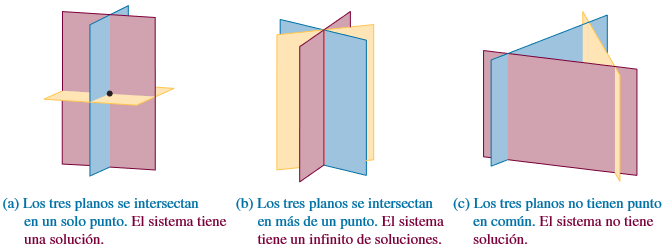
\includegraphics[scale=0.65]{img/number_of_solutions.png}
\caption{Stewart, et. al (2017). \textit{Precálculo. Matemáticas para el Cálculo}. Pp. 643.}
\end{figure}

También un sistema de $3 \times 3$ no tiene solución si ninguno de los tres planos se intersectan\footnote{En el caso (c) que vemos en la imagen, al menos dos planos se intersectan, pero también puede darse el caso en el que ninguno se toque. Ambos casos significan que el sistema no tiene solución.}.

\subsection{Soluciones de un Sistema Lineal Cuadrado usando Matrices.}

La clase anterior vimos que un sistema de ecuaciones lineales podemos representarlo de forma matricial como:
\[
  \mathbf{A} \mathbf{x} = \mathbf{b}
\]
Si el sistema lineal es cuadrado, la matriz de coeficientes $\mathbf{A}$ también lo será y, por tanto, podemos buscar su inversa. Si $\mathbf{A}^{-1}$ existe, es posible garantizar que el sistema tiene \textbf{una única solución}, la cual es dada por:
\[
  \mathbf{x} = \mathbf{A}^{-1} \mathbf{b}
\]
En un sistema de $3 \times 3$, si $\mathbf{A}^{-1}$ existe significa que los tres planos se intersectan en un solo punto. No obstante, esta matriz no siempre es posible encontrarla.

Recordemos que $\exists \mathbf{A}^{-1} \iff \det(\mathbf{A}) \neq 0$. Este es el criterio de invertibilidad y lo vimos reflejado en la fórmula para obtener la matriz inversa usando la matriz adjunta de $\mathbf{A}$.
\[
  \mathbf{A}^{-1} = \frac{1}{\det(\mathbf{A})} \text{Adj}(\mathbf{A})
\]
Si, en caso contrario, el $\det(\mathbf{A}) = 0$, $\mathbf{A}^{-1}$ no existe\footnote{Sea que la busquemos usando la matriz adjunta o por eliminación de Gauss, el valor del determinante nos dirá si existe o no esta matriz.}. Para el caso de un sistema lineal de $3 \times 3$ se traduce en que:

\begin{enumerate}
\item tenga infinitas soluciones (los planos se cruzan en una misma recta) o
\item no tenga solución.
\end{enumerate}

Veamos, como ejemplo, el siguiente \textbf{sistema homogéneo de ecuaciones lineales}\footnote{Un sistema homogéneo es aquel donde los valores de la derecha de las ecuaciones son \textbf{iguales a cero}.}:
\[
\left\{
\begin{aligned}
x + z = 0 \\
x + y = 0 \\
x + 2y + 3z = 0
\end{aligned}
\right.
\]
Un sistema homogéneo siempre es consistente (i.e, siempre tendrá al menos una solución) porque se cumplen las igualdades para el punto $(0, \ 0, \ 0)$, también conocido como ``solución trivial''.

Por lo tanto, quedan dos posibilidades: que el sistema tenga una única solución o tenga infinitas (i.e, más de una). El primer caso lo podemos conocer si comprobamos que existe $\mathbf{A}^{-1}$ a partir del determinante de $\mathbf{A}$ siendo distinto de cero. Si esto ocurre, significa que:
\begin{align*}
  \mathbf{A} \mathbf{x} &= \mathbf{0} \\
             \mathbf{x} &= \mathbf{A}^{-1} \cdot \mathbf{0} \\
             \mathbf{x} &= \mathbf{0}
\end{align*}
donde $\mathbf{0}$ es el vector cero. Gráficamente quiere decir que \textbf{los tres planos se intersectan en el origen}.

De igual modo, el segundo caso también es posible conocerlo por medio del determinante de $\mathbf{A}$, pero cuando éste es igual a cero. En dicha instancia, \textbf{los planos se intersectan en una misma recta tomando infinitos puntos}, la cual \textbf{pasa por el origen} porque es una de las soluciones del sistema.

Otra forma de entender que un sistema homogéneo lineal de $3 \times 3$ tiene infinitas soluciones cuando el $\det(\mathbf{A}) = 0$, es considerar que las filas de $\mathbf{A}$ corresponden a los vectores normales de las tres ecuaciones. Esto significa que:
\[
  \det(\mathbf{A}) = \det(\mathbf{n}_{1}, \ \mathbf{n}_{2}, \ \mathbf{n}_{3}) = 0
\]
En la Clase 2 vimos que el valor absoluto del determinante de tres vectores en $\mathbb{R}^{3}$ es equivalente al volumen de un paralelepipedo. Si este es igual a cero, quiere decir que aquel sólido es un plano (i.e, sin volumen) donde $\mathbf{n}_{1}$, $\mathbf{n}_{2}$ y $\mathbf{n}_{3}$ son \textbf{coplanares}\footnote{Es decir, pertenecen al mismo plano.}.

Por lo tanto, si graficamos a los tres vectores normales en sus planos y calculamos el producto cruz entre dos de ellos, el vector resultante estará en la dirección de la recta en la que se intersectan los tres planos. Es decir, la recta de las soluciones será perpendicular al plano formado por los vectores normales y paralelo a los planos. Esto significa, además, que con dicho producto podemos conocer las soluciones.

Así, un sistema $\mathbf{A}\mathbf{x} = \mathbf{b}$ cualquiera de $3 \times 3$ y considerando el $\det(\mathbf{A})$, podemos resumir sus soluciones de la siguiente manera:

\begin{table}[hbt!]
\centering

\begin{tabular}{c c c c}
\hline
$\det(\mathbf{A})$ & Cantidad de Soluciones & Solución & Intersección de los tres planos \\
\hline
$\neq 0$ & Una & $\mathbf{x} = \mathbf{A}^{-1} \mathbf{b}$ & En un punto \\
$= 0$ & Infinitas & - & En una recta \\
$= 0$ & Ninguna & - & No coinciden en un lugar \\
\hline
\end{tabular}

\end{table}


\end{document}
